\documentclass[11pt]{article}

\usepackage[a4paper, margin=0.85in]{geometry}
\usepackage{graphicx}
\usepackage{array}
\usepackage{hyperref}
\usepackage{enumitem}
\usepackage{caption}
\usepackage{helvet}
\usepackage{xcolor}
\usepackage{tabularx}
\usepackage{tikz}
\usetikzlibrary{arrows.meta, positioning, shapes.geometric}

\newcolumntype{C}[1]{>{\centering\arraybackslash}p{#1}}
\newcolumntype{L}[1]{>{\raggedright\arraybackslash}p{#1}}

\renewcommand{\familydefault}{\sfdefault}
\setlength{\parindent}{0pt}
\setlength{\parskip}{0.48em}
\setlist[itemize]{leftmargin=*, itemsep=0.2em}
\setlist[enumerate]{leftmargin=*, itemsep=0.25em}
\hypersetup{
    colorlinks=true,
    linkcolor=black,
    urlcolor=blue
}

\pagestyle{plain}

\newcommand{\screenimage}[3]{
\begin{figure}[h]
    \centering
    \includegraphics[width=#3\textwidth]{#2}
    \caption*{#1}
\end{figure}
}

\newcommand{\smallcell}[1]{\small #1}

\begin{document}

\begin{center}
    \textbf{\Huge NUS Orbital 2026}

    \vspace{1.0cm}

    
\includegraphics[width=0.32\textwidth]{team_logo.jpg}

    \vspace{0.7cm}

    \textbf{\LARGE Milestone 01 Artemis Resubmission}

    \vspace{0.7cm}

    {\Large
    \underline{\href{https://drive.google.com/file/d/1kHCFBJZEATOGSeAxe3MZQu1tjgT1XCv5/view?usp=share_link}{Poster}}
    \hspace{0.2cm}
    \underline{\href{https://drive.google.com/file/d/1g0qcSA1oe-XH0mgNVUuB4pHMQPBQDxpa/view?usp=share_link}{Video Walkthrough}}
    \hspace{0.2cm}
    \underline{\href{https://orbital-artemis-armap-nus.onrender.com}{Deployed App}}
    \hspace{0.2cm}
    \underline{\href{https://github.com/77chenchen/Orbital_Artemis_ArMap_Nus/issues}{GitHub Logs}}
    }

    \vspace{0.9cm}

    \textbf{\LARGE Atlas (Team ID: \hspace{2.2cm})}\\
    {\large Wang Qichen (A0337219B)}\\
    {\large Feng Yi (A0322277E)}

    \vspace{0.5cm}

    \textbf{\large Proposed Level of Achievement: Artemis}
\end{center}

\newpage

\tableofcontents

\newpage

\section*{Resubmission Response}
\addcontentsline{toc}{section}{Resubmission Response}

This report has been rewritten for Artemis Milestone 01 re-evaluation. The previous submission did not clearly demonstrate Artemis-level planning, project-level software engineering, automated testing, CI/CD, and walkthrough evidence. This version makes those items explicit and connects them to the current codebase, deployed application, and GitHub workflow.

\begin{center}
\renewcommand{\arraystretch}{1.28}
\begin{tabularx}{\textwidth}{|C{0.08\textwidth}|L{0.33\textwidth}|X|}
\hline
\textbf{No.} & \textbf{Expectation} & \textbf{Where Addressed In This Report} \\
\hline
1 & 20--23 user stories & The User Stories section contains 22 stories grouped by student, route, facility, schedule, accessibility, administrator, and engineering personas. \\
\hline
2 & Ideation for all \(\geq 9\) features & The Feature Ideation section describes 10 planned or implemented features, each with problem, idea, Milestone 01 status, and later extension. \\
\hline
3 & Project-level software engineering & The Software Engineering At Project Level section documents GitHub issues, PRs, module boundaries, branch policy, dependency management, environment management, and risk handling. \\
\hline
4 & Artemis M1 page depth & The report has been expanded beyond the previous Apollo-like summary and is compiled as a full Artemis M1 technical report. \\
\hline
5 & Automated testing documentation & The Testing Strategy section documents automated checks, manual regression tests, and current test limitations. \\
\hline
6 & CI/CD setup and documentation & A GitHub Actions workflow has been added at \texttt{.github/workflows/ci.yml}; the CI/CD section documents frontend build, backend tests, Docker build, and deployment path. \\
\hline
7 & Video walkthrough & The Video Walkthrough section states what the submitted video demonstrates and links it from the cover page. \\
\hline
\end{tabularx}
\end{center}

\section*{Deployment and Submitted Materials}
\addcontentsline{toc}{section}{Deployment and Submitted Materials}

The deployed web application is available at:
\href{https://orbital-artemis-armap-nus.onrender.com}{orbital-artemis-armap-nus.onrender.com}.

The GitHub repository and issue tracker are available at:
\href{https://github.com/77chenchen/Orbital_Artemis_ArMap_Nus}{Atlas GitHub repository}.

The submitted video walkthrough is linked on the cover page. It is intended to show the app as a working prototype, not just a code repository: login, protected access, campus dashboard, map rendering, mobile layout, and the current user flow are demonstrated in sequence.

\newpage

\section*{Motivation}
\addcontentsline{toc}{section}{Motivation}

Navigating NUS is difficult for new students, exchange students, visitors, and even current students moving between unfamiliar faculties. Public maps may show buildings, but students often need more than a building polygon: they need to know which entrance to use, whether the building has facilities they need, how long it may take to move there, and whether their next class or meeting changes the priority of route suggestions.

Atlas is motivated by the gap between static campus maps and the real decision-making students perform every day. A student does not simply ask ``where is COM2?'' The more realistic question is: ``I am currently at one location, I have class soon, I may need a bus, and I need to know the most useful next action.'' Atlas therefore combines authentication, campus map rendering, facility discovery, schedule awareness, bus context, and a daily assistant interface.

\section*{Aim and Artemis Scope}
\addcontentsline{toc}{section}{Aim and Artemis Scope}

Atlas aims to become a campus assistant for NUS students that supports map-based navigation, facility discovery, schedule-aware guidance, and future AR-style indoor navigation. For Artemis Milestone 01, our goal is not only to produce a working prototype, but also to establish a project foundation that can scale into later milestones.

For this milestone, we focus on:

\begin{itemize}
    \item a deployed full-stack application using React, Go, SQLite, and Docker;
    \item authentication with email/password, demo mode, protected routes, JWTs, and Google Sign-In;
    \item campus data APIs for buildings, facilities, schedules, recommendations, sync status, and bus context;
    \item MapLibre/OpenStreetMap rendering and early route-oriented interactions;
    \item mobile usability and an iOS app shell;
    \item project-level engineering practices: GitHub issues, branches, pull requests, CI, build checks, and deployment documentation.
\end{itemize}

\newpage

\section*{User Stories}
\addcontentsline{toc}{section}{User Stories}

The 22 user stories below define the wider Artemis product vision. Milestone 01 implements the first layer of this vision and creates a platform for later AR, indoor mapping, and personalization work.

\begin{enumerate}
    \item As a new NUS student, I want to search for a campus building by name so that I can find unfamiliar locations quickly.
    \item As a student rushing to class, I want route guidance from my current location to a target building so that I can arrive on time.
    \item As a student with back-to-back lessons, I want Atlas to consider my schedule so that it can highlight the next relevant destination.
    \item As a student inside an unfamiliar building, I want to find facilities such as restrooms, lifts, study spaces, and printers so that I can solve immediate needs.
    \item As a student with accessibility needs, I want lift and accessible-route information so that I can avoid unsuitable paths.
    \item As an exchange student, I want building and facility names to be searchable without knowing exact abbreviations so that I can navigate NUS confidently.
    \item As a student using a phone outdoors, I want the interface to be readable on mobile so that I can use the app while walking.
    \item As a student with limited mobile data, I want the app to load essential map and schedule information efficiently so that navigation remains practical.
    \item As a student planning my day, I want to add and remove schedule items so that Atlas can reflect my actual timetable.
    \item As a student leaving a lecture, I want recommendations for nearby useful resources so that I can decide what to do next.
    \item As a student using NUS shuttle buses, I want bus stop and arrival context so that I can decide whether to walk or take a bus.
    \item As a student who values privacy, I want login-protected access so that personal schedule data is not exposed publicly.
    \item As a returning user, I want a persistent account flow so that I do not need to re-enter setup information every time.
    \item As a user who wants to try the project quickly, I want demo mode so that I can evaluate Atlas without creating a full account.
    \item As a user with a Google account, I want Google Sign-In so that login is faster and closer to real student authentication patterns.
    \item As a project evaluator, I want a deployed app URL so that I can inspect the prototype without local setup.
    \item As a project evaluator, I want a video walkthrough so that I can understand feature usability without guessing from screenshots.
    \item As a developer, I want frontend and backend modules to be separated so that map, auth, and data work can progress independently.
    \item As a developer, I want CI checks on pull requests so that broken builds and backend regressions are caught before merge.
    \item As a developer, I want environment variables documented so that local and production setups are reproducible.
    \item As a maintainer, I want seeded demo data so that the application can be tested consistently.
    \item As a future Artemis team member, I want a foundation for AR and indoor navigation so that later milestones can build on working map, auth, and data layers.
\end{enumerate}

\newpage

\section*{Feature Ideation}
\addcontentsline{toc}{section}{Feature Ideation}

The table below records ideation for 10 features. Each feature is treated as part of the product plan, not only as an isolated implementation task.

\begin{center}
\renewcommand{\arraystretch}{1.25}
\begin{tabularx}{\textwidth}{|C{0.055\textwidth}|L{0.19\textwidth}|X|X|}
\hline
\textbf{No.} & \textbf{Feature} & \textbf{Ideation and User Value} & \textbf{M1 Status and Later Extension} \\
\hline
1 & Repository foundation & Create a reproducible full-stack project with clear ownership between frontend, backend, deployment, and documentation. & Implemented. Later work adds stricter PR templates and release tags. \\
\hline
2 & Email and demo login & Let students and evaluators enter the app through either real credentials or a low-friction demo path. & Implemented with JWT flow. Later work adds password reset and stronger account management. \\
\hline
3 & Google Sign-In & Support a realistic student login path using a trusted identity provider. & Implemented through frontend ID token submission and backend verification. Later work can connect to NUS identity if available. \\
\hline
4 & Protected dashboard & Keep schedule and personalized recommendations behind an authentication boundary. & Implemented with protected frontend routes and backend authorization headers. \\
\hline
5 & Campus data dashboard & Present buildings, facilities, schedules, recommendations, and sync status in a student-facing workspace. & Implemented with seeded SQLite data and API endpoints. Later work expands data coverage. \\
\hline
6 & Map rendering & Provide an interactive campus map instead of static screenshots. & Implemented with MapLibre and OSM-style map rendering. Later work adds richer indoor overlays. \\
\hline
7 & Search and route tracing & Allow users to move from typed destination intent to route-oriented map interaction. & Partially implemented through search, markers, and route drawing. Later work improves routing accuracy. \\
\hline
8 & NUS bus context & Include campus transit as part of navigation decisions. & Implemented as bus stops, routes, arrivals, active vehicles, alerts, and context endpoints with demo fallback. \\
\hline
9 & Mobile and iOS shell & Make the app usable in the realistic mobile setting where navigation happens. & Implemented responsive UI and Capacitor iOS shell. Later work can add native plugins. \\
\hline
10 & CI/CD and deployment & Make engineering quality visible through automated checks and reproducible deployment. & CI added through GitHub Actions; deployment documented for Render and Docker/Caddy. \\
\hline
\end{tabularx}
\end{center}

\newpage

\section*{Overall Architecture}
\addcontentsline{toc}{section}{Overall Architecture}

The architecture follows a modular system design: user interface, authentication, campus assistant/dashboard, map/navigation, backend APIs, persistent data, and external services. This is important at project level because each module can evolve without rewriting the whole system.

\begin{figure}[h]
    \centering
    \resizebox{\textwidth}{!}{%
    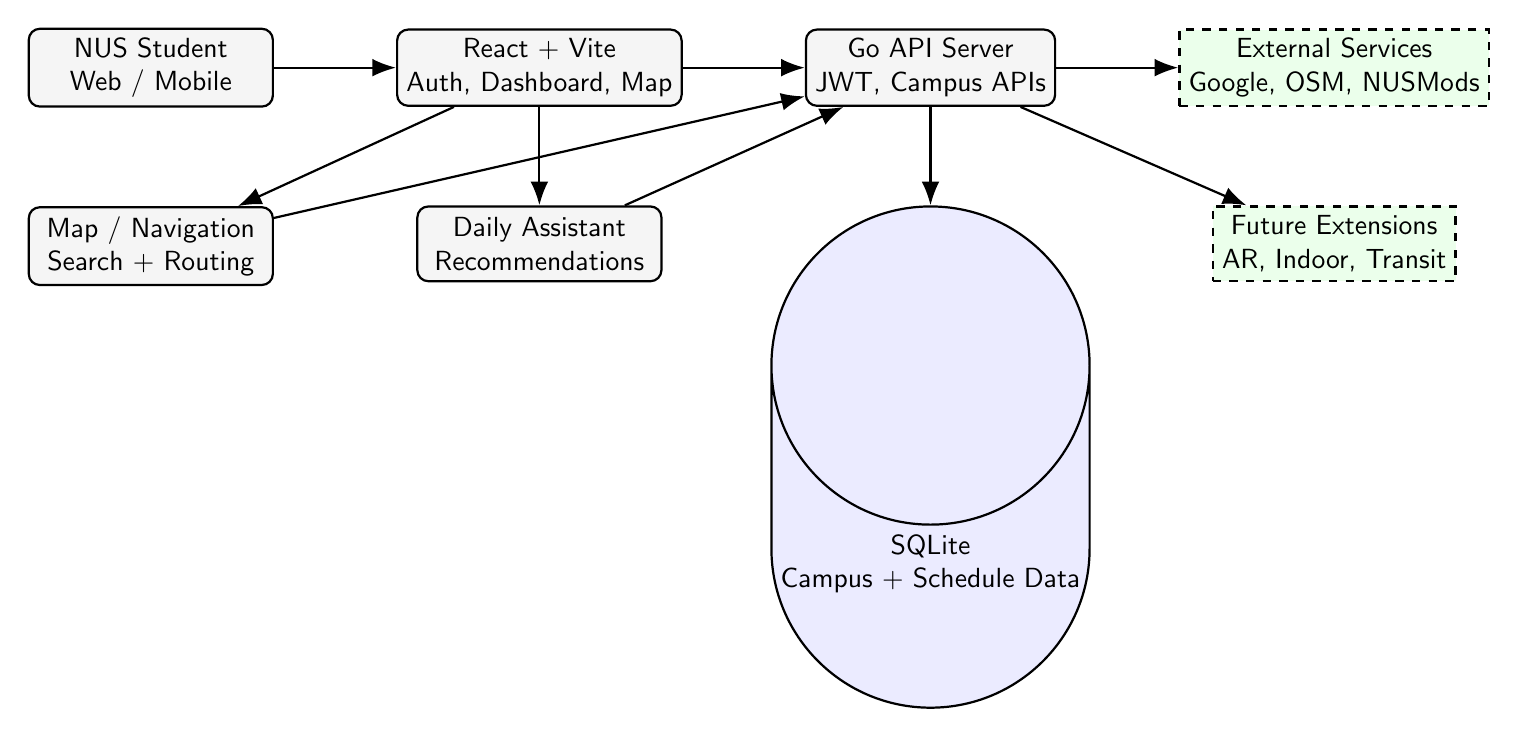
\begin{tikzpicture}[
        node distance=1.25cm and 1.55cm,
        box/.style={rectangle, rounded corners, draw=black, thick, align=center, minimum width=3.1cm, minimum height=0.95cm, fill=gray!8},
        data/.style={cylinder, shape border rotate=90, draw=black, thick, align=center, minimum width=2.7cm, minimum height=1.1cm, fill=blue!8},
        ext/.style={rectangle, draw=black, dashed, thick, align=center, minimum width=2.9cm, minimum height=0.9cm, fill=green!8},
        arrow/.style={-{Latex[length=3mm]}, thick}
    ]
        \node[box] (user) {NUS Student\\Web / Mobile};
        \node[box, right=of user] (frontend) {React + Vite\\Auth, Dashboard, Map};
        \node[box, right=of frontend] (backend) {Go API Server\\JWT, Campus APIs};
        \node[data, below=of backend] (db) {SQLite\\Campus + Schedule Data};
        \node[box, below=of frontend] (assistant) {Daily Assistant\\Recommendations};
        \node[box, below=of user] (map) {Map / Navigation\\Search + Routing};
        \node[ext, right=of backend] (external) {External Services\\Google, OSM, NUSMods};
        \node[ext, below=of external] (future) {Future Extensions\\AR, Indoor, Transit};

        \draw[arrow] (user) -- (frontend);
        \draw[arrow] (frontend) -- (backend);
        \draw[arrow] (backend) -- (db);
        \draw[arrow] (backend) -- (external);
        \draw[arrow] (frontend) -- (assistant);
        \draw[arrow] (frontend) -- (map);
        \draw[arrow] (assistant) -- (backend);
        \draw[arrow] (map) -- (backend);
        \draw[arrow] (backend) -- (future);
    \end{tikzpicture}
    }
    \caption*{Atlas overall architecture}
\end{figure}

\newpage

\section*{Software Engineering At Project Level}
\addcontentsline{toc}{section}{Software Engineering At Project Level}

\subsection*{Project Structure}
\addcontentsline{toc}{subsection}{Project Structure}

\begin{figure}[h]
    \centering
    \fbox{
        \begin{minipage}{0.88\textwidth}
            \vspace{0.6em}
            {\small\ttfamily
            \mbox{\detokenize{Orbital_Artemis_ArMap_Nus/}}\\
            \mbox{\detokenize{|-- frontend/              React + Vite frontend and mobile app shell}}\\
            \mbox{\detokenize{|   |-- src/               Auth, dashboard, campus map, and UI code}}\\
            \mbox{\detokenize{|   `-- ios/               Capacitor iOS project}}\\
            \mbox{\detokenize{|-- backend/               Go API server}}\\
            \mbox{\detokenize{|   |-- cmd/server/        Server entry point}}\\
            \mbox{\detokenize{|   `-- internal/atlas/    Auth, campus data, routing, and API logic}}\\
            \mbox{\detokenize{|-- deploy/                Caddy and production deployment notes}}\\
            \mbox{\detokenize{|-- .github/workflows/     CI workflow for build, test, and Docker image}}\\
            \mbox{\detokenize{|-- Dockerfile             Production image definition}}\\
            \mbox{\detokenize{|-- docker-compose.yml     Local production-like stack}}\\
            \mbox{\detokenize{`-- readme.tex             Milestone report source}}
            }
            \vspace{0.2em}
        \end{minipage}
    }
    \caption*{Project structure}
\end{figure}

\subsection*{Project Management}
\addcontentsline{toc}{subsection}{Project Management}

The team uses GitHub issues as the task log, feature branches for isolated work, and pull requests for integration. Issues are used not only as a checklist, but also as a planning surface: authentication, map rendering, search, dashboard integration, mobile usability, bus integration, and deployment are separated into trackable units. This prevents the project from becoming a single unreviewable prototype.

At project level, Atlas applies these principles:

\begin{itemize}
    \item \textbf{Separation of concerns:} React owns user interaction; Go owns authentication, data APIs, and trusted external calls; SQLite owns seeded persistent state.
    \item \textbf{Reproducibility:} README, Dockerfile, Docker Compose, and environment variables document how to run the same app locally or in production.
    \item \textbf{Incremental delivery:} Milestone 01 establishes auth, dashboard, map, bus, deployment, and mobile shell before attempting heavier AR features.
    \item \textbf{Risk reduction:} uncertain future work such as indoor AR is postponed until map, data, and identity foundations are reliable.
    \item \textbf{Reviewability:} feature branches and PRs keep map changes, auth changes, and deployment changes inspectable.
\end{itemize}

\newpage

\section*{Implemented Core Features}
\addcontentsline{toc}{section}{Implemented Core Features}

\subsection*{Authentication and Protected Access}
\addcontentsline{toc}{subsection}{Authentication and Protected Access}

Authentication allows students to enter Atlas through email/password login, registration, demo mode, or Google Sign-In. Once authenticated, users can access protected pages such as the dashboard and map.

\screenimage{Authentication Screen}{readme_assets/authentication-login-page.png}{0.94}

On the backend, Atlas verifies credentials and issues a JWT. For Google Sign-In, the frontend obtains a Google ID token and sends it to the backend, where it is verified against the configured Google client ID. The backend then returns the same application JWT format used by email login, keeping the rest of the application independent of the authentication method.

\subsection*{Campus Dashboard and Assistant}
\addcontentsline{toc}{subsection}{Campus Dashboard and Assistant}

The dashboard connects campus data to the student's daily context. Instead of showing raw database rows, Atlas groups buildings, facilities, schedules, recommendations, NUSMods sync status, and bus information into sections that can be scanned quickly.

This feature is important for Artemis because it moves the project beyond a simple map. The assistant layer is where later schedule-aware navigation, reminders, and AR hints can be connected.

\subsection*{Campus Map Rendering}
\addcontentsline{toc}{subsection}{Campus Map Rendering}

The map feature gives users an interactive visual interface for campus navigation. Atlas renders a MapLibre/OpenStreetMap-based campus map centered around NUS and prepares the surface for future indoor overlays and AR markers.

\screenimage{Campus Map Screen}{readme_assets/campus-map-screen.png}{0.94}

The map logic is separated into a map initialization module, a \texttt{MapEngine} helper, routing services, and UI components. This modular approach prevents the main map page from becoming a large untestable component.

\newpage

\section*{Implemented Supporting Features}
\addcontentsline{toc}{section}{Implemented Supporting Features}

\subsection*{Location Search and Route Interaction}
\addcontentsline{toc}{subsection}{Location Search and Route Interaction}

Location search improves usability by allowing users to type a destination instead of manually inspecting the map. Selecting a suggestion places a marker and moves the map to the chosen location. Route tracing then allows selected start and end points to be drawn on the map as an early prototype of the navigation goal.

The state is split into display text and confirmed place objects. This simple model-view separation avoids treating incomplete text as a real geospatial endpoint.

\subsection*{NUS Bus Context}
\addcontentsline{toc}{subsection}{NUS Bus Context}

Atlas includes NUS bus endpoints for stops, routes, arrivals, active vehicles, alerts, and location-based bus context. When live API credentials are not configured, the backend can serve demo data. This design keeps local development usable while still preparing for real campus transit integration.

\subsection*{Mobile and iOS Experience}
\addcontentsline{toc}{subsection}{Mobile and iOS Experience}

Campus navigation is often used while students are moving, so mobile usability is not optional. The frontend is designed to remain readable on common mobile widths, and a Capacitor iOS shell under \texttt{frontend/ios} loads the deployed HTTPS app.

\begin{figure}[h]
    \centering
    \begin{minipage}{0.44\textwidth}
        \centering
        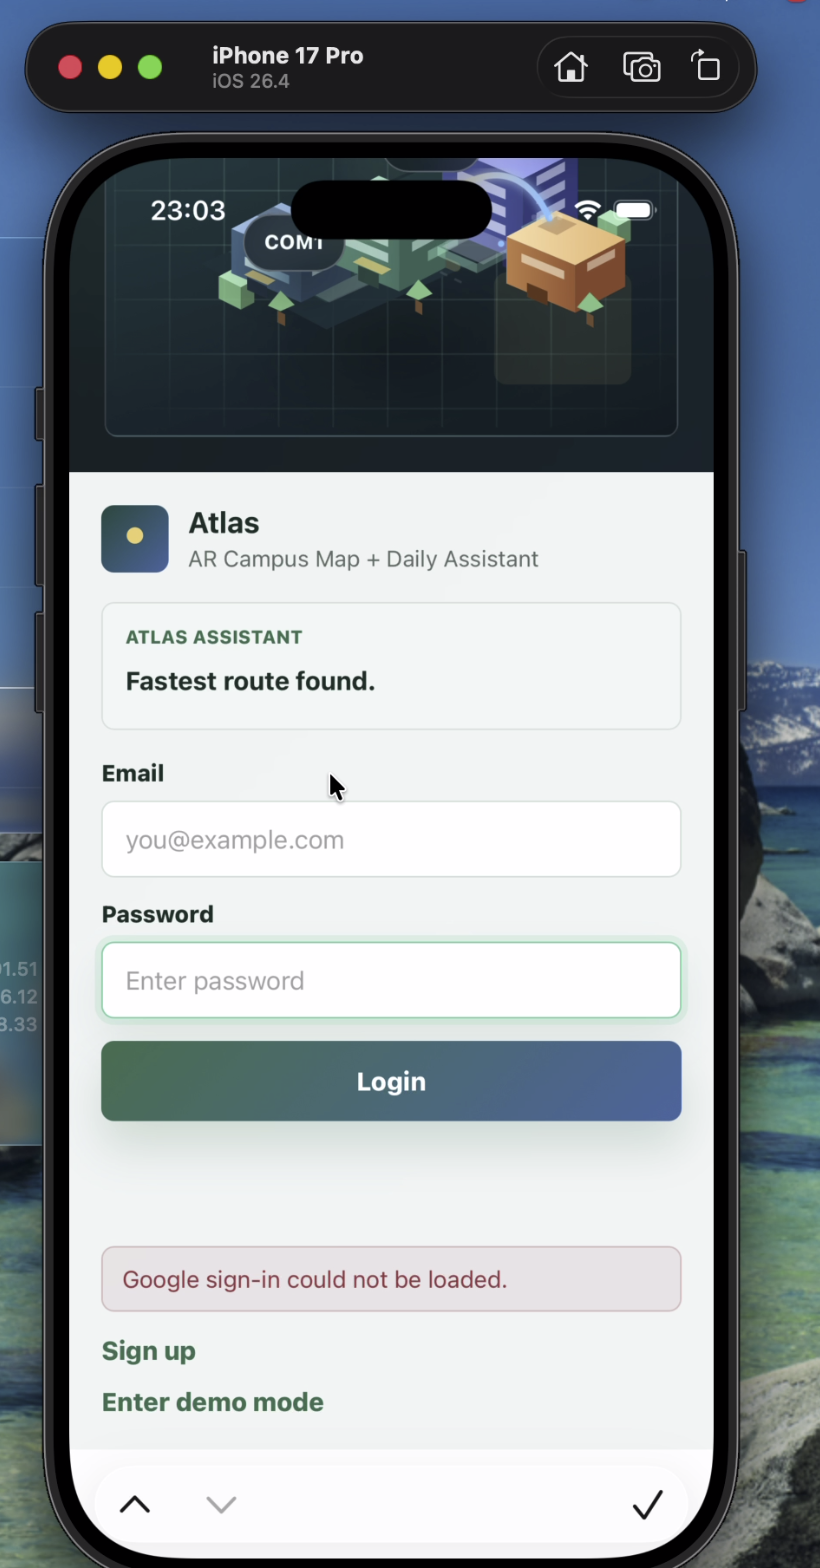
\includegraphics[width=0.88\textwidth]{readme_assets/mobile-app-1.png}
    \end{minipage}
    \hfill
    \begin{minipage}{0.44\textwidth}
        \centering
        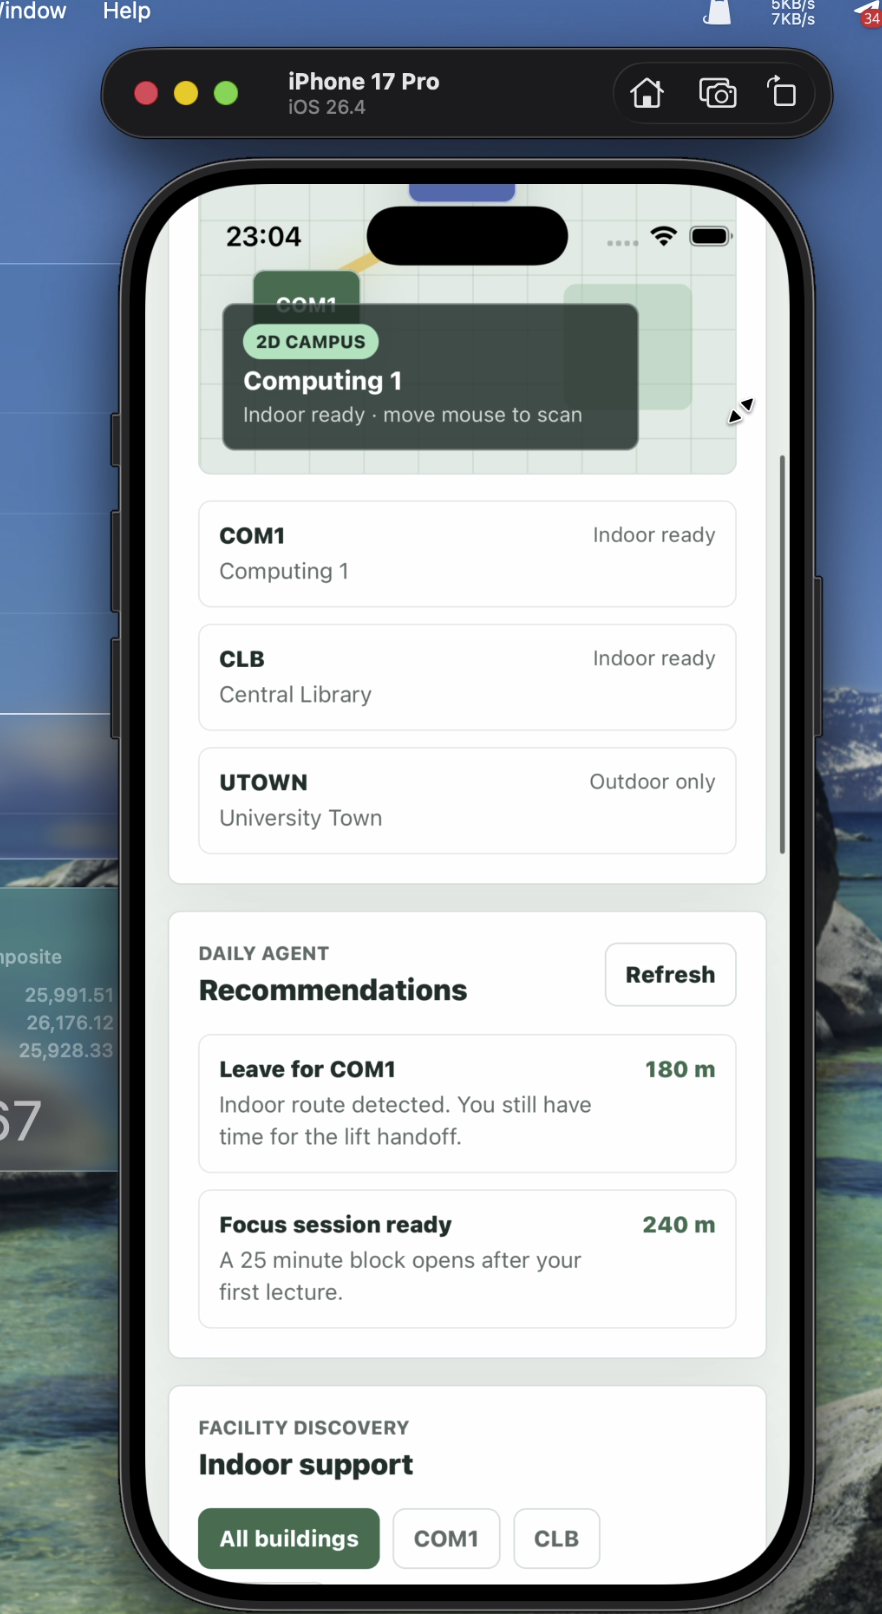
\includegraphics[width=0.88\textwidth]{readme_assets/mobile-app-2.png}
    \end{minipage}
    \caption*{Mobile app screens}
\end{figure}

\newpage

\section*{Testing Strategy}
\addcontentsline{toc}{section}{Testing Strategy}

Testing is documented as both automated checks and manual regression checks. The current codebase is still a Milestone 01 prototype, so the automated layer focuses on build and backend correctness gates, while manual checks cover user-facing workflows that are difficult to validate without a browser session.

\subsection*{Automated Checks}
\addcontentsline{toc}{subsection}{Automated Checks}

\begin{center}
\renewcommand{\arraystretch}{1.25}
\begin{tabularx}{\textwidth}{|L{0.23\textwidth}|L{0.28\textwidth}|X|}
\hline
\textbf{Check} & \textbf{Command / Location} & \textbf{Purpose} \\
\hline
Frontend production build & \texttt{cd frontend \&\& npm run build} & Confirms that the React/Vite app bundles successfully and catches broken imports or invalid build-time code. \\
\hline
Backend Go test gate & \texttt{cd backend \&\& go test ./...} & Compiles all backend packages and runs Go tests as they are added. This catches API, auth, store, and scheduler regressions at package level. \\
\hline
Docker production image & \texttt{docker build -t atlas-ci .} & Confirms the production image can be built from the repository without relying on local developer state. \\
\hline
CI workflow & GitHub Actions & Runs the frontend build, backend tests, and Docker build from \texttt{ci.yml} on push and pull requests to \texttt{main}. \\
\hline
\end{tabularx}
\end{center}

\subsection*{Manual Regression Checks}
\addcontentsline{toc}{subsection}{Manual Regression Checks}

\begin{center}
\renewcommand{\arraystretch}{1.2}
\begin{tabularx}{\textwidth}{|L{0.25\textwidth}|X|}
\hline
\textbf{Workflow} & \textbf{Manner of Testing} \\
\hline
Login and registration & Test demo login, email login, registration, invalid credentials, and protected-route redirection. \\
\hline
Google Sign-In & Test that the frontend obtains an ID token and the backend exchanges it for an app JWT. \\
\hline
Dashboard data & Verify buildings, facilities, schedule cards, recommendations, and sync status load after authentication. \\
\hline
Map rendering & Open the campus map and verify map tiles, NUS centering, markers, and route drawing behavior. \\
\hline
Bus context & Verify stops, routes, arrival cards, active vehicles, and demo fallback behavior when live credentials are absent. \\
\hline
Mobile layout & Use narrow browser viewport and iOS shell to confirm content does not overflow and main actions remain reachable. \\
\hline
Deployment smoke test & Open the Render deployment and check that frontend routes and backend APIs are served together. \\
\hline
\end{tabularx}
\end{center}

Known limitation: Milestone 01 currently has stronger automated build gates than fine-grained unit tests. In the next milestone, the team will add focused tests for authentication handlers, schedule CRUD, recommendation logic, bus fallback behavior, and frontend interaction flows.

\newpage

\section*{CI/CD Pipeline}
\addcontentsline{toc}{section}{CI/CD Pipeline}

A CI workflow has been added to the repository at \texttt{.github/workflows/ci.yml}. It runs on push and pull requests targeting \texttt{main}. This directly supports Artemis expectations because code quality is checked at project level rather than only through local manual testing.

\begin{figure}[h]
    \centering
    \resizebox{\textwidth}{!}{%
    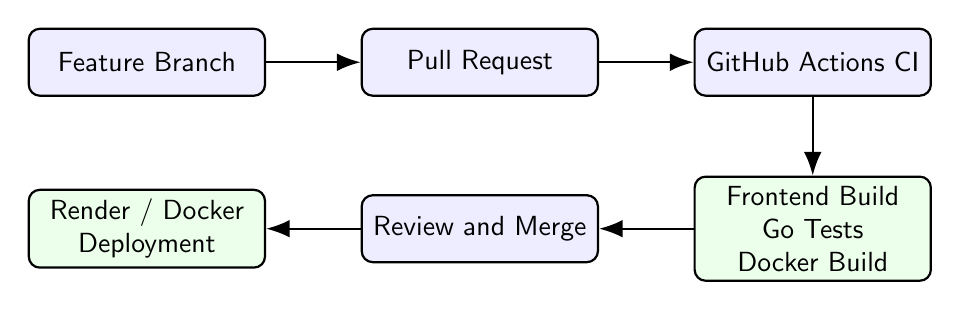
\begin{tikzpicture}[
        node distance=1.0cm and 1.2cm,
        box/.style={rectangle, rounded corners, draw=black, thick, align=center, minimum width=3.0cm, minimum height=0.85cm, fill=blue!7},
        ok/.style={rectangle, rounded corners, draw=black, thick, align=center, minimum width=3.0cm, minimum height=0.85cm, fill=green!8},
        arrow/.style={-{Latex[length=3mm]}, thick}
    ]
        \node[box] (branch) {Feature Branch};
        \node[box, right=of branch] (pr) {Pull Request};
        \node[box, right=of pr] (ci) {GitHub Actions CI};
        \node[ok, below=of ci] (checks) {Frontend Build\\Go Tests\\Docker Build};
        \node[box, left=of checks] (review) {Review and Merge};
        \node[ok, left=of review] (deploy) {Render / Docker\\Deployment};

        \draw[arrow] (branch) -- (pr);
        \draw[arrow] (pr) -- (ci);
        \draw[arrow] (ci) -- (checks);
        \draw[arrow] (checks) -- (review);
        \draw[arrow] (review) -- (deploy);
    \end{tikzpicture}
    }
    \caption*{Atlas CI/CD pipeline}
\end{figure}

The CI jobs are:

\begin{itemize}
    \item \textbf{Frontend build:} installs dependencies in \texttt{frontend/} with \texttt{npm ci} and runs \texttt{npm run build}.
    \item \textbf{Backend tests:} uses the Go version from \texttt{backend/go.mod}, downloads modules, and runs \texttt{go test ./...}.
    \item \textbf{Docker build:} builds the production image after frontend and backend jobs pass.
\end{itemize}

The deployment path is documented through the Render-hosted app and the Docker/Caddy production stack. The intended release discipline is: work on feature branch, open PR, pass CI, merge to \texttt{main}, then deploy from the stable branch.

\newpage

\section*{UML Diagrams}
\addcontentsline{toc}{section}{UML Diagrams}

\subsection*{Authentication Flow}
\addcontentsline{toc}{subsection}{Authentication Flow}

\begin{figure}[h]
    \centering
    \resizebox{0.88\textwidth}{!}{%
    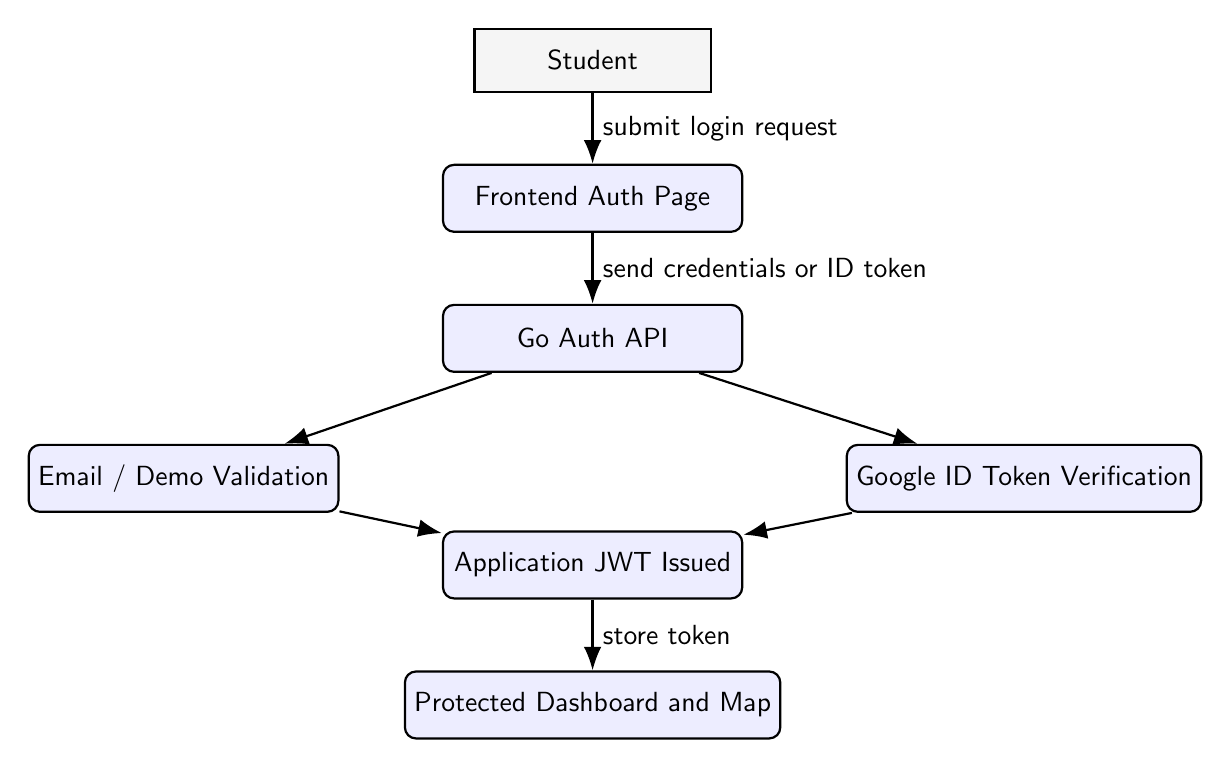
\begin{tikzpicture}[
        node distance=0.9cm and 1.3cm,
        actor/.style={rectangle, draw=black, thick, align=center, minimum width=3.0cm, minimum height=0.8cm, fill=gray!8},
        proc/.style={rectangle, rounded corners, draw=black, thick, align=center, minimum width=3.8cm, minimum height=0.85cm, fill=blue!7},
        arrow/.style={-{Latex[length=3mm]}, thick}
    ]
        \node[actor] (student) {Student};
        \node[proc, below=of student] (frontend) {Frontend Auth Page};
        \node[proc, below=of frontend] (backend) {Go Auth API};
        \node[proc, below left=of backend] (local) {Email / Demo Validation};
        \node[proc, below right=of backend] (google) {Google ID Token Verification};
        \node[proc, below=2.0cm of backend] (jwt) {Application JWT Issued};
        \node[proc, below=of jwt] (protected) {Protected Dashboard and Map};

        \draw[arrow] (student) -- node[right]{submit login request} (frontend);
        \draw[arrow] (frontend) -- node[right]{send credentials or ID token} (backend);
        \draw[arrow] (backend) -- (local);
        \draw[arrow] (backend) -- (google);
        \draw[arrow] (local) -- (jwt);
        \draw[arrow] (google) -- (jwt);
        \draw[arrow] (jwt) -- node[right]{store token} (protected);
    \end{tikzpicture}
    }
    \caption*{Authentication sequence for protected access}
\end{figure}

\subsection*{Map Search and Routing Flow}
\addcontentsline{toc}{subsection}{Map Search and Routing Flow}

\begin{figure}[h]
    \centering
    \resizebox{\textwidth}{!}{%
    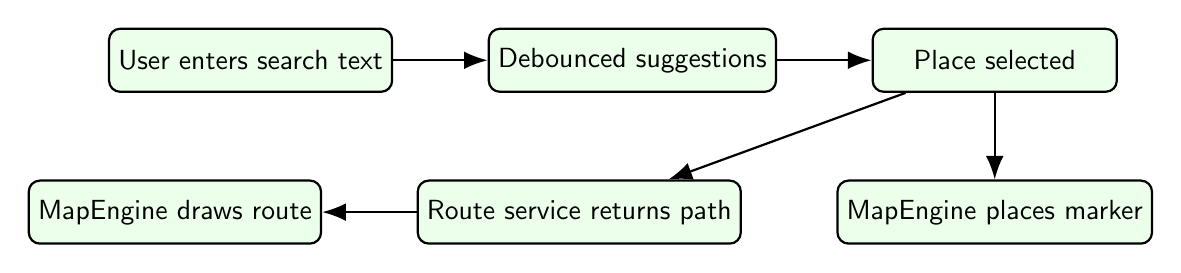
\begin{tikzpicture}[
        node distance=1.1cm and 1.2cm,
        box/.style={rectangle, rounded corners, draw=black, thick, align=center, minimum width=3.1cm, minimum height=0.8cm, fill=green!8},
        arrow/.style={-{Latex[length=3mm]}, thick}
    ]
        \node[box] (input) {User enters search text};
        \node[box, right=of input] (suggest) {Debounced suggestions};
        \node[box, right=of suggest] (select) {Place selected};
        \node[box, below=of select] (marker) {MapEngine places marker};
        \node[box, left=of marker] (route) {Route service returns path};
        \node[box, left=of route] (draw) {MapEngine draws route};

        \draw[arrow] (input) -- (suggest);
        \draw[arrow] (suggest) -- (select);
        \draw[arrow] (select) -- (marker);
        \draw[arrow] (select) -- (route);
        \draw[arrow] (route) -- (draw);
    \end{tikzpicture}
    }
    \caption*{Map search and route drawing workflow}
\end{figure}

\newpage

\section*{Video Walkthrough}
\addcontentsline{toc}{section}{Video Walkthrough}

The video link is included on the cover page as ``Video Walkthrough.'' The walkthrough is structured to demonstrate usability instead of only showing code. It covers:

\begin{itemize}
    \item opening the deployed app from the public URL;
    \item entering through login or demo mode;
    \item reaching protected dashboard content after authentication;
    \item viewing campus data, schedule context, recommendations, and sync status;
    \item opening the campus map and demonstrating map-centered navigation behavior;
    \item showing mobile responsiveness through current mobile screenshots or viewport demonstration;
    \item explaining how the current prototype prepares for later AR and indoor navigation milestones.
\end{itemize}

This directly addresses the earlier weakness that the submission did not sufficiently demonstrate current feature usability.

\section*{Milestone 01 Progress}
\addcontentsline{toc}{section}{Milestone 01 Progress}

Milestone 01 now provides a working React frontend, Go backend, SQLite data layer, authentication flow, campus dashboard, map page, bus endpoints, mobile shell, deployment path, and CI workflow. The project is still early, but it is no longer only an ideation artifact: it is a deployed, inspectable, and build-checked prototype.

\section*{Planned Next Steps}
\addcontentsline{toc}{section}{Planned Next Steps}

\begin{itemize}
    \item Add backend unit tests for login, registration, schedule CRUD, recommendation generation, and bus demo fallback.
    \item Add frontend interaction tests for login, protected routing, dashboard rendering, and map controls.
    \item Expand campus data coverage for rooms, entrances, lifts, accessible routes, and indoor facilities.
    \item Improve route accuracy with multimodal walking and shuttle-bus routing.
    \item Turn the iOS shell into a more native mobile experience if required by later milestones.
    \item Continue user validation with NUS students and refine the assistant workflow from feedback.
    \item Prepare AR-style indoor navigation only after stable data, routing, and mobile foundations are in place.
\end{itemize}

\end{document}
